 \documentclass[final,3p,times,10pt,onecolumn]{myElsarticle}
\usepackage{float}
\usepackage{times}
\usepackage[utf8]{inputenc}
\usepackage[english]{babel}
\usepackage[T1]{fontenc}
\usepackage{geometry}
\usepackage{color}
\usepackage{soul}
\usepackage{cancel}
\usepackage{subfigure}
\usepackage{enumerate}
\usepackage{amsmath,amsthm,amsfonts,amssymb}
\usepackage{amsthm}
\usepackage{graphicx}
\graphicspath{{./figs/}}
\numberwithin{equation}{section}
\usepackage{spverbatim}
\usepackage{fancyhdr}
\usepackage{listings} 
\usepackage{lineno}
\usepackage[none]{hyphenat}
\date{\today}
\setcounter{secnumdepth}{3}
\providecommand{\abs}[1]{\lvert#1\rvert}
\providecommand{\norm}[1]{\lVert#1\rVert}
\setlength\parindent{12pt}		

\linenumbers

\newcommand{\COM}[1]{{\color{green} #1}}
\newcommand{\HA}[1]{{\color{red} #1}}
\newcommand{\CIP}[1]{{\color{blue} #1}}
\newcommand{\CMV}[1]{{\color{orange} #1}}


\begin{document}

\begin{frontmatter}

\title{A second-order approximation on SIMPLEC: the COMPLEX algorithm}
%% A second-neighbor extended correction for segregated p-v coupling algorithms
 
\author[a,e]{Horacio J. Aguerre}
\author[b,a]{Cesar I. Pairetti}
\author[a,b]{Cesar M. Venier}
\author[a,c]{Santiago Marquez Damian}
\author[a,d]{Norberto M. Nigro}

\address[a]{Centro de Investigación de Métodos Computacionales, CONICET-UNL, Santa Fe, Argentina}
\address[b]{Escuela de Ingenier\'ia Mec\'anica, Facultad de Ciencias Exactas, Ingenieria y Agrimensura, Universidad Nacional de Rosario, Rosario, Argentina}
\address[c]{Facultad Regional Santa Fe, Universidad Tecnologica Nacional, Santa Fe, Argentina}
\address[d]{Facultad de Ingeniería y Ciencias Hídricas, Universidad Nacional del Litoral, Santa Fe, Argentina}
\address[e]{Facultad Regional Concepción de Uruguay, Universidad Tecnologica Nacional, Concepción del Uruguay, Argentina}

%Start of abstract
\begin{abstract}
a
\end{abstract}

\begin{keyword}
Segregated algorithms \sep Segregated method \sep Collocated grids \sep Finite Volume Method 
\end{keyword}
\end{frontmatter}

%%%%%%%%%%%%%%%%%%%%%%%%%%%%%%%%%%%%%
\section{Introduction}

\begin{enumerate}
    \item {\color{red} Introducción a CFD en FVM, metodos de acoplamiento p-v: Monolitico vs Segregados. Relevancia de los metodos segregados.} 
    \item {\color{red} Establecer problemática de los segregados: costo computacional de iterar. Variantes respecto a SIMPLE y objetivos de cada variante: SIMPLE con relajación de P, SIMPLEC mejora sobre SIMPLE, PISO mejora sobre SIMPLE}
    \item {\color{red} Introduccion a COMPLEX, que motivo esta propuesta, en que se basa, problematica que viene a solucionar}
    \item {\color{red} Descripcion de las secciones del paper.}
\end{enumerate}

\section{Theoretical background} \label{sec:theory}

\subsection{The SIMPLE algorithm on collocated grids}

The continuum incompressible Navier-Stokes equations may be presented as:

\begin{equation}
\displaystyle \nabla \cdotp \boldsymbol{u} = 0, 
\label{eq:mass1}
\end{equation}

\begin{equation}
\displaystyle \frac{\partial \boldsymbol{u}}{\partial t} + \nabla \cdotp (\boldsymbol{u} \boldsymbol{u}) = -\nabla p + \nu\, \nabla^2 \boldsymbol{u} + \boldsymbol{\Phi},
\label{eq:mom1}
\end{equation}

\noindent where $\displaystyle p = \frac{\mathcal{P}}{\rho}$, $\mathcal{P}$ is the pressure field, $\boldsymbol{u} = (u,v,w)$ is the velocity field, {\color{red}$\rho$ is the mass density, }$\nu$ is the kinematic viscosity and $\mathbf{\Phi}$ is a momentum source term (e.g. a body force).
Based on the Finite Volume Method \cite{jasak}, Eqs.~(\ref{eq:mass1}) and~(\ref{eq:mom1}) may be discretized as:

\begin{equation}
\begin{split}
\sum_{f} \boldsymbol{u}_{f} \cdotp \textbf{S}_{f} = \sum_{f} F_f = 0, 
\end{split}
\label{eq:mass2} 
\end{equation}

\begin{equation}
\begin{split}
a_P\,\boldsymbol{u}_P + \sum_{N} a_{N}\,\boldsymbol{u}_{N} = b_P\, \boldsymbol{u}^0_P + \boldsymbol{\Phi}_P - \nabla p_P,
\label{eq:umom1}
\end{split}
\end{equation}

\noindent where the subscript $P$ indicates the cell-centered value of the current cell, $N$ indicates neighbor cells values and $f$ refers to the face values. The term ${\color{red}b_P}\, \boldsymbol{u}^0_P$ is the contribution of the previous time-step and is function of the temporal scheme. {\color{red} The face-normal vector $\textbf{S}_{f}$ has the magnitude of the face area and points out of the cell}, $F_f$ is the {\color{red} velocity} flux at the face $f$ and $a_P$ and $a_{N}$ are the diagonal and off-diagonal momentum matrix coefficients respectively. The operator $\nabla p_P$ is a Gauss-based gradient of the pressure computed using first neighbors values of that field. Isolating $\boldsymbol{u}_P$ from Eq.~(\ref{eq:umom1}),

\begin{equation}
\begin{split}
\boldsymbol{u}_P = \frac{1}{a_P}\left(b_P\, \boldsymbol{u}^0_P + \boldsymbol{\Phi}_P - \sum_{N} a_{N}\, \boldsymbol{u}_{N} - \nabla p_P\right),
\label{eq:uP}
\end{split}
\end{equation}

One way to solve Eqs. (\ref{eq:mass2}) and (\ref{eq:umom1}) for $\boldsymbol{u}$ and $p$ consists on addressing one equation at a time, update one of the unknown fields, solve the remaining equation and iterate the sequence. These techniques are known as segregated methods, where the SIMPLE-family techniques \cite{patankar1972,patankar1980,patankar1981,vanDoormal,issa} are among the most popular for incompressible flows. It broadly consists of a Momentum Predictor step and a Corrector step. In the Momentum Predictor, a first approximation for the velocity field is computed using the momentum equation where the pressure term is treated explicitly. 
{\color{red}
\begin{equation} \label{eq:MOMPRED}
\begin{split}
a_P\, \boldsymbol{u}_P^{*} = \boldsymbol{H}^* - \nabla p_P^{*}%, \\
%p_P^* &= p_P^0
\end{split}
\end{equation}

\CIP{En este punto podríamos meter la definición de H si es que queremos escribir todo "a la FOAM". Me parece más natural escribir en términos de $u$, así se ve más claro cómo entra la aproximación de los vecinos usando el gradiente de velocidad}

\noindent where 

\begin{equation}
\boldsymbol{H}^* = - \sum_N a_N \boldsymbol{u}_N^* + \boldsymbol{\Phi}_P    
\end{equation}

\noindent and the superscript $0$ indicates fields that are stored from previous iterations and $*$ are the fields being solved at the current iteration. }
This preliminary result does not satisfy the divergence-free condition in Eq. (\ref{eq:mass2}). In the Corrector step, a pressure correction is computed from an equation based on including the momentum equation, as expressed in Eq. (\ref{eq:uP}), in the mass conservation  Eq. (\ref{eq:mass2}). In this context, the velocity correction can be expressed in the following manner

\CIP{A continuación desarrollo las ecuaciones de forma relativa. Hay que definir si queda así o en términos absoultos (como FOAM). La ventaja del $H$ es que Rhie Chow queda implícito (acá no está hecho) y que FOAM labura así.}

\begin{align}
\label{eq:uprimeDef}
\boldsymbol{u}_P^{**} &= \boldsymbol{u}_P^{*} + \boldsymbol{u}_P^{'} \\
\qquad \boldsymbol{u}_P^{'} &= \frac{1}{a_P}\left(\boldsymbol{H}'- \nabla p_P^{'}\right).
\end{align}

\noindent where,

\begin{align}
\label{eq:HPrima}
   \boldsymbol{H}' = - \sum_N a_N \boldsymbol{u}'_N 
\end{align}

Then, the divergence-free condition can be expressed in terms of the previous expressions

\begin{align} \label{eq:div-free1}
\nabla \cdot \left(\boldsymbol{u}_P^{*} + \boldsymbol{u}_P^{'}\right) &= 0 \\
\sum_f \left(\boldsymbol{u_P}'\right)_{f} \cdot \boldsymbol{S}_f &= -\sum_f \left(\boldsymbol{u_P}^{*}\right)_{f} \cdot \boldsymbol{S}_f \label{eq:div-free2} \\
\sum_f \left[\frac{1}{a_P}\left(\boldsymbol{H}' - \nabla p_P^{'}\right)\right]_f\cdot \boldsymbol{S}_f &= -\sum_f \left[\frac{1}{a_P}\left(\boldsymbol{H}^* - \nabla p_P^{*}\right)\right]_f \cdot \boldsymbol{S}_f \label{eq:div-free3}
\end{align}

%\noindent where, $\boldsymbol{u}^*_f$ is obtained by linear interpolation of the $\boldsymbol{u}^*_{P}$ values on the cells that shares the same face $f$.

%The system of equations given by \ref{eq:div-free} for all the cells is highly coupled due to the presence of the corrections on the neighbors. To reduce the computational effort, the SIMPLE algorithm introduce the assumption that $\boldsymbol{u}'_N$ are negligible. With this simplification, the system turns to be

The SIMPLE method considers $\boldsymbol{H}'=\boldsymbol{0}$, thus Eq.~(\ref{eq:div-free2}) becomes:

\begin{equation}
\sum_f 
\left[
\frac{1}{a_P}
\left(
-
\nabla p_P^{'}
\right)
\right]_f\cdot \boldsymbol{S}_f 
=
-\sum_f \left[\frac{1}{a_P}\left(\boldsymbol{H}^* - \nabla p_P^{*}\right)\right]_f \cdot
\boldsymbol{S}_f.
\label{eq:div-free4}    
\end{equation}
Then, grouping the pressure terms, a relation based on $p^{**}$ is obtained,
\begin{equation}
\sum_f 
\left[
\frac{1}{a_P}
\left(
\nabla p_P^{**}
\right)
\right]_f\cdot \boldsymbol{S}_f 
=
\sum_f 
\left[
\frac{1}{a_P}
\left(
\boldsymbol{H}^*
\right)
\right]_f
\cdot
\boldsymbol{S}_f.
\label{eq:div-free5}  
\end{equation}

% \begin{equation}
% \label{eq:pEqnSIMPLE1}
% \sum_f \left(\frac{1}{a_P}\right)_f \nabla p_f^{'}  \cdot \boldsymbol{S}_f= \sum_f \left[\frac{1}{a_P}\left(\boldsymbol{H}^* - \nabla p_P^{*}\right)\right]_f \cdot \boldsymbol{S}_f
% \end{equation}

% (acá hay que escribir algun bolazo de porque distribuimos la interpolación en el producto)

\noindent which is a Poisson problem that has the pressure correction values as unknowns. Nevertheless, solving this system in a straightforward manner may lead to high-frequency oscillations. The Rhie-Chow correction \cite{rhiechow} reduces this effect in collocated grids, 

\begin{equation}
\label{eq:pEqnSIMPLE2}
\sum_f 
\left[
\frac{1}{a_P}
\left(
\nabla p_P^{**}
\right)
\right]_f\cdot \boldsymbol{S}_f 
=
\sum_f 
\left[
\frac{1}{a_P}
\left(
\boldsymbol{H}^*
\right)
\right]_f
\cdot
\boldsymbol{S}_f 
+
\sum_f  
\left[
\left(
\frac{\nabla p_P^{**}}{a_P}
\right)_f
- 
\left(
\frac{1}{a_P}
\right)_f 
\nabla p_f^{**} 
\right]
\cdot 
\boldsymbol{S}_f 
\end{equation}

 Finally, the pressure equation can be written as:



\begin{equation}\label{eq:pEqnSIMPLE3}
\sum_f \left(\frac{1}{a_P}\right)_f \nabla p_f^{**} \cdot \boldsymbol{S}_f =  \sum_f \left(\frac{\boldsymbol{H}^*}{a_P}\right)_f \cdot \boldsymbol{S}_f 
\end{equation}

\noindent where,

\begin{equation}
 p_P^{'} = p_P^{**} - p_P^{*}
\end{equation}

The corrected velocity value is then given by

\begin{equation}\label{eq:SIMPLECorr}
\boldsymbol{u}_P^{**} = \boldsymbol{u}_P^* - \frac{\nabla p_P'}{a_P}.
\end{equation}

\iffalse
 In order to do so, the velocity field $\boldsymbol{u}_P$, originally on cell-centers, needs to be interpolated to the faces obtaining: 

 \begin{equation}
 \begin{split}
 \sum_{f} \left( \boldsymbol{H}_P - \frac{1}{a_P} \nabla p_P  \right)_f \cdotp \textbf{S}_{f} = 0 
 \end{split}
 \label{eq:pEq1} 
 \end{equation}

Therefore, the Corrector step may be summarized as:

\begin{enumerate}

\item Assemble and solve the pressure based on Eq.~(\ref{eq:pEq1}):

\begin{equation}
\begin{split}
\sum_{f} \left( \frac{1}{a_P} \nabla p'_P \right)_f \cdotp \textbf{S}_{f} = \sum_{f} \boldsymbol{u}^*_f \cdotp \textbf{S}_{f}
\end{split}
\label{eq:pEq2} 
\end{equation}


%\CIP{Si conservamos la forma relativa, aquí habría que meter la explicación de Rhie Chow}

\item {\color{red}Compute} the face fluxes by adding the new pressure contribution:

\begin{equation}
\begin{split}
F_f = \boldsymbol{u}^*_f \cdotp \textbf{S}_{f} -  \left( \frac{1}{a_P}\right)_f \nabla p'_f  \cdotp \textbf{S}_{f}
\end{split}
\label{eq:Fhat} 
\end{equation}

\item Correct the cell-centered velocity field based on the new pressure field, using Eq. (\ref{eq:umom3b})

\begin{equation}\label{eq:umom3b}
\begin{split}
\boldsymbol{u}_P = \boldsymbol{u}^*_P - \frac{1}{a_P} \nabla p'_P 
\end{split}
\end{equation}

\end{enumerate}

\fi
Most of the SIMPLE-family algorithms preserve this general structure. In particular, the SIMPLE algorithm \cite{patankar1972}, originally conceived as a steady state flow solver, adds under-relaxation factors to obtain a stable solution. Another variant is the PISO {\color{red}(Pressure-Implicit with Splitting of Operators)} algorithm, which relies on iterating the Corrector step a given number of times to ensure a correct coupling between pressure and velocity for transient flow problems \cite{issa,issa2}. {\color{red} The SIMPLE-PISO combined technique has been largely adopted in several computational codes (e.g. OpenFOAM(R) \cite{ofpg}) to address transient incompressible flow problems due to its beneficial convergence features. It consists on iterating the corrector steps until a certain mass conservation criteria is fulfilled (as in PISO) and iterating the whole sequence (Momentum Predictor and Corrector Step) several times until both mass and momentum equations are verified for each time step. This algorithm will be adopted in the present work.}

\subsection{Improving the neighbor approximation: the SIMPLEC algorithm}
The SIMPLEC~\cite{vanDoormal} algorithm proposes an aproximation of the neighbour velocity correction $\boldsymbol{u}_N'$,
\begin{equation}
\label{Eq:simplecAproximation}
\boldsymbol{u}_N'
=
\boldsymbol{u}_P'
\end{equation}
Based on last assumption the Eq.~(\ref{eq:HPrima}) may be expressed as,

\begin{equation}\label{eq:H_SIMPLEC}
\boldsymbol{H}'= \left(-\sum_N a_N\right) \boldsymbol{u}'_P,
\end{equation}

\noindent which can be computed and included in the momentum equation leading to:

\begin{align}\label{eq:uPrimeSIMPLEC}
a_P\,\boldsymbol{u}_P^{'} &= -\boldsymbol{u}'_P \sum_{N} a_{N}\ - \nabla p_P^{'}
\end{align}

\noindent and then

\begin{align}\label{eq:uPrimeSIMPLEC2}
 \boldsymbol{u}_P^{'} &= - \frac{\nabla p_P^{'}}{a_P + \sum_{N} a_{N}}
\end{align}


The following equivalence is defined,
\begin{equation}
\tilde{a}_p 
\equiv
a_P + \sum_{N} a_{N},
\end{equation}
Then:

\begin{align}\label{eq:uPrimeSIMPLEC2}
\boldsymbol{u}_P^{'} 
=
- 
\dfrac
{
\nabla p_P^{'}
}
{
\tilde{a_P}
}
\end{align}

Including this expression into Eq.~(\ref{eq:div-free2}):

\begin{align} 
\sum_f \left(\boldsymbol{u_P}'\right)_{f} \cdot \boldsymbol{S}_f &= -\sum_f \left(\boldsymbol{u_P}^{*}\right)_{f} \cdot \boldsymbol{S}_f \label{eq:div-free4}
\end{align}
\noindent the following pressure equation is obtained:

\begin{equation}
\label{eq:pEqnSIMPLEC1}
\sum_f 
\left[
\left(
\frac
{
1
}
{
\tilde{a}_P
}
\right)
\nabla p_P^{'}
\right]_f
\cdot 
\boldsymbol{S}_f
= 
\sum_f 
\left[
\frac{1}{a_P}
\left(
\boldsymbol{H}^* - \nabla p_P^{*}
\right)
\right]_f 
\cdot
\boldsymbol{S}_f.
\end{equation}


Adding the following term  in both terms of previous equation
\begin{equation}
\sum_f
\left[
\left(
\dfrac
{1}
{\tilde{a}_P}
\right)
\nabla p^*
\right]_f
 \cdot S_f,
\end{equation}
 and grouping the pressure terms,
\begin{equation}
\label{eq:pEqnSIMPLEC1}
\sum_f 
\left[
\left(
\frac
{
1
}
{
\tilde{a}_P
}
\right)
\nabla p_P^{**}
\right]_f
\cdot 
\boldsymbol{S}_f
= 
\sum_f 
\left[
\frac{1}{a_P}
\left(
\boldsymbol{H}^*
\right)
\right]_f 
\cdot
\boldsymbol{S}_f
+
\sum_f
\left[
\left(
\dfrac{1}
{\tilde{a}_P}
-
\dfrac{1}
{a_P}
\right)
\nabla p^*
\right]_f
\cdot
\boldsymbol{S}_f
\end{equation}


The pressure equation is obtained by including an analogous Rhie-Chow correction:

\begin{equation}
\begin{split}
\label{eq:pEqnSIMPLEC2}
\sum_f 
\left[
\left(
\frac
{
1
}
{
\tilde{a}_P
}
\right)
\nabla p_P^{**}
\right]_f
\cdot 
\boldsymbol{S}_f
=
\\ 
\sum_f 
\left[
\frac{1}{a_P}
\left(
\boldsymbol{H}^*
\right)
\right]_f 
\cdot
\boldsymbol{S}_f
+
\sum_f
\left[
\left(
\dfrac{1}
{\tilde{a}_P}
-
\dfrac{1}
{a_P}
\right)
\nabla p^*
\right]_f
\cdot
\boldsymbol{S}_f
+
\sum_f
\left\lbrace
\left(
\dfrac
{
\nabla p^{**}
}
{\tilde{a}_P}
\right)_f
-
\left(
\dfrac
{1}
{\tilde{a}_P}
\right)_f
\nabla p^{**}_f
+
\left(
\dfrac
{1}
{\tilde{a}_P}
-
\dfrac
{1}
{a_P}
\right)_f
\nabla p^{*}_f
-
\left[
\left(
\dfrac
{1}
{\tilde{a}_P}
-
\dfrac
{1}
{a_P}
\right)
\nabla p^*
\right]_f
\right\rbrace
\cdot
S_f
\end{split}
\end{equation}
Then, simplifying,
\begin{equation}
\sum_f
\left[
\left(
\dfrac
{1}
{\tilde{a}_P}
\right)_f
\nabla p^{**}_f
\right]
\cdot 
\boldsymbol{S}_f
= 
\sum_f 
\left[
\frac{1}{a_P}
\left(
\boldsymbol{H}^*
\right)
\right]_f 
\cdot
\boldsymbol{S}_f
+
\sum_f
\left[
\left(
\dfrac
{1}
{\tilde{a}_P}
-
\dfrac
{1}
{a_P}
\right)_f
\nabla p^{*}_f
\right]
\cdot
\boldsymbol{S}_f
\end{equation}


Then, the velocity correction may be computed as follows:

\begin{equation}\label{eq:uCorrSIMPLEC}
\boldsymbol{u}^{**}_P = \boldsymbol{u}_P^* - \frac{\nabla p_P^{'}}{\tilde{a}_P}.
\end{equation}

Last equation may be expressed also by means of the $H^*$ operator,
\begin{equation}
\boldsymbol{u}^{**}_P 
=
\dfrac
{\boldsymbol{H}_P^* }
{a_P}
- 
\frac{\nabla p_P^{*}}{a_P}
- 
\frac{\nabla p_P^{'}}{\tilde{a}_P}.
\end{equation}
which may be considered including absolute pressure values,
\begin{equation}
\boldsymbol{u}^{**}_P 
=
\dfrac
{\boldsymbol{H}_P^* }
{a_P}
- 
\frac{\nabla p_P^{**}}{\tilde{a}_P}
+
\left(
\dfrac{1}{\tilde{
a}_P}
-
\dfrac{1}{a_P}
\right)
\nabla p_P^{*}.
\end{equation}


The only difference between SIMPLE and SIMPLEC are the coefficients in the Corrector step. Nevertheless, this slight modification shows a significant improvement in the stability  and convergence properties of the algorithm \cite{liu}. In the spirit of using better approximation for the neighbors correction values, we propose the following method.

\section{Enhancement of SIMPLEC: the COMPLEX method}
\label{sec:COMPLEX}

In order to estimate the value of $\boldsymbol{u}_N'$ in Eq.~(\ref{eq:HPrima}), a second order Taylor approximation is proposed,
\begin{equation}\label{eq:uNTaylor}
\boldsymbol{u}_N' = \boldsymbol{u}_P' + \boldsymbol{x}_{PN}\cdot 
\nabla \boldsymbol{u}_f'.
\end{equation}

Replacing Eq.~(\ref{eq:uNTaylor}) in (\ref{eq:HPrima}), considering the same velocity gradient for all the neighbor approximations
\begin{align}
\label{eq:uPrimeCOMPLEX}
a_P\,\boldsymbol{u}_P^{'} 
&=
 -\sum_{N} a_{N}\, \left(\boldsymbol{u}_P^{'} + \boldsymbol{x}_{PN}\cdot \nabla \boldsymbol{u}_f'\right)- \nabla p_P^{'}, 
\\
\boldsymbol{u}_P^{'} 
&=
- \dfrac{\nabla p_P^{'}}
{\tilde{a}_P}
-
\dfrac
{
\sum_{N} a_{N} 
( 
\boldsymbol{x}_{PN} 
\cdot
\nabla \boldsymbol{u}_f' 
)
}
{\tilde{a}_P}.
\end{align}

\begin{align} 
\label{eq:div-free4Again}
\sum_f \left(\boldsymbol{u_P}'\right)_{f} \cdot \boldsymbol{S}_f &= -\sum_f \left(\boldsymbol{u_P}^{*}\right)_{f} \cdot \boldsymbol{S}_f 
\end{align}

\begin{equation}
\label{eq:pEqnCOMPLEX1}
\sum_f 
\left[
\left(
\frac
{
1
}
{
\tilde{a}_P
}
\right)
\nabla p_P^{'}
\right]_f
\cdot 
\boldsymbol{S}_f
= 
\sum_f 
\left[
\frac{1}{a_P}
\left(
\boldsymbol{H}^* - \nabla p_P^{*}
\right)
\right]_f 
\cdot
\boldsymbol{S}_f
-
\sum_f 
\left[
\dfrac
{
\sum_{N} a_{N} 
( 
\boldsymbol{x}_{PN} 
\cdot
\nabla \boldsymbol{u}_f' 
)
}
{\tilde{a}_P}
\right]_f 
\cdot
\boldsymbol{S}_f.
\end{equation}

\begin{equation}
\label{Eq:complexSemiFinal}
\sum_f
\left[
\left(
\dfrac
{1}
{\tilde{a}_P}
\right)_f
\nabla p^{**}_f
\right]
\cdot 
\boldsymbol{S}_f
= 
\sum_f 
\left[
\frac{1}{a_P}
\left(
\boldsymbol{H}^*
\right)
\right]_f 
\cdot
\boldsymbol{S}_f
+
\sum_f
\left[
\left(
\dfrac
{1}
{\tilde{a}_P}
-
\dfrac
{1}
{a_P}
\right)_f
\nabla p^{*}_f
\right]_f
\cdot
S_f
-
\sum_f 
\left[
\dfrac
{
\sum_{N} a_{N} 
( 
\boldsymbol{x}_{PN} 
\cdot
\nabla \boldsymbol{u}_f' 
)
}
{\tilde{a}_P}
\right]_f 
\cdot
\boldsymbol{S}_f
\end{equation}

\subsection{Computation of the face gradient}
The face gradient $\nabla \boldsymbol{u}_f' $ is obtained as a linear interpolation of a cell-centred gradient,
\begin{equation}
\label{Eq:UFaceGradient}
\nabla \boldsymbol{u}_f'
=
(\nabla \boldsymbol{u}_P')_f.
\end{equation}
To obtain $\nabla \boldsymbol{u}_P'$, the face values $\boldsymbol{u_P}'_f$ of the mass balance of Eq.~(\ref{eq:div-free4Again}) are expressed as a  first-order Taylor expansion,
\begin{equation}
\label{Eq:TaylorOnFace}
\left(
\boldsymbol{u_P}'
\right)_f
=
\boldsymbol{u_P}'
+
\boldsymbol{x}_{Pf}
\cdot 
\nabla \boldsymbol{u}_P'.
\end{equation} 


Subsequently, this last equation is replaced in  Eq.~(\ref{eq:div-free4Again}),
\begin{align}
\sum_f 
\left(
\boldsymbol{u_P}'
+
\boldsymbol{x}_{Pf}
\cdot 
\nabla \boldsymbol{u}_P'
\right)
\cdot 
\boldsymbol{S}_f 
&=
-\sum_f
\left(
\boldsymbol{u_P}^{*}
\right)_{f} 
\cdot 
\boldsymbol{S}_f
\\
\boldsymbol{u_P}'
\cdot 
\sum_f 
\boldsymbol{S}_f
+
\sum_f 
\left(
\boldsymbol{x}_{Pf}
\cdot 
\nabla \boldsymbol{u}_P'
\right)
\cdot 
\boldsymbol{S}_f
&=
-\sum_f
\left(
\boldsymbol{u_P}^{*}
\right)_{f} 
\cdot 
\boldsymbol{S}_f
\\
\label{Eq:Last}
\sum_f 
\left(
\boldsymbol{x}_{Pf}
\cdot 
\nabla \boldsymbol{u}_P'
\right)
\cdot 
\boldsymbol{S}_f
&=
-\sum_f
\left(
\boldsymbol{u_P}^{*}
\right)_{f} 
\cdot 
\boldsymbol{S}_f
\end{align}

where,
\begin{equation}
\left(
\boldsymbol{u_P}^{*}
\right)_{f}
=
\left[\frac{1}{a_P}\left(\boldsymbol{H}^* - \nabla p_P^{*}\right)\right]_f
\end{equation}

Then, a similar form of the Rhie-Chow term given in Eq.~(\ref{eq:pEqnSIMPLE2}) is included,
\begin{equation}
\left(
\boldsymbol{u_P}^{*}
\right)_{f}
=
\left[\frac{1}{a_P}\left(\boldsymbol{H}^* - \nabla p_P^{*}\right)\right]_f
+
\left[
\left(
\frac{\nabla p_P^{*}}{a_P}
\right)_f
- 
\left(
\frac{1}{a_P}
\right)_f 
\nabla p_f^{*} 
\right]
\end{equation}

Simplifying, 
\begin{equation}
\left(
\boldsymbol{u_P}^{*}
\right)_{f}
=
 \left(\frac{\boldsymbol{H}^*}{a_P}\right)_f 
 -
 \left(\frac{1}{a_P}\right)_f \nabla p_f^{*}
\end{equation}

Replacing in Eq.~(\ref{Eq:Last}),
\begin{equation}
\sum_f 
\left(
\boldsymbol{x}_{Pf}
\cdot 
\nabla \boldsymbol{u}_P'
\right)
\cdot 
\boldsymbol{S}_f
=
-\sum_f
\left[
\left(\frac{\boldsymbol{H}^*}{a_P}\right)_f 
 -
 \left(\frac{1}{a_P}\right)_f \nabla p_f^{*}
 \right]
\cdot 
\boldsymbol{S}_f
\end{equation}
The following assumption is proposed:
\begin{equation}
\nabla \boldsymbol{u}_P'
=
\alpha
\boldsymbol{I}
\end{equation}

Replacing,
\begin{align}
\sum_f 
\left(
\boldsymbol{x}_{Pf}
\cdot 
\alpha
\boldsymbol{I}
\right)
\cdot 
\boldsymbol{S}_f
&=
-\sum_f
\left[
\left(\frac{\boldsymbol{H}^*}{a_P}\right)_f 
 -
 \left(\frac{1}{a_P}\right)_f \nabla p_f^{*}
 \right]
\cdot 
\boldsymbol{S}_f
\\
\alpha
\sum_f 
\left(
\boldsymbol{x}_{Pf}
\cdot 
\boldsymbol{I}
\right)
\cdot 
\boldsymbol{S}_f
&=
-\sum_f
\left[
\left(\frac{\boldsymbol{H}^*}{a_P}\right)_f 
 -
 \left(\frac{1}{a_P}\right)_f \nabla p_f^{*}
 \right]
\cdot 
\boldsymbol{S}_f,
\end{align}
then
\begin{equation}
\alpha
=
\dfrac
{-\sum_f
\left[
\left(\frac{\boldsymbol{H}^*}{a_P}\right)_f 
 -
 \left(\frac{1}{a_P}\right)_f \nabla p_f^{*}
 \right]
\cdot 
\boldsymbol{S}_f}
{\sum_f 
\boldsymbol{x}_{Pf}
\cdot 
\boldsymbol{S}_f}
\end{equation}

Finally the face gradient~(\ref{Eq:UFaceGradient}) may be computed using the $\alpha$ values on the faces,
\begin{equation}
\nabla \boldsymbol{u}_f'
=
\alpha_f
\boldsymbol{I}.
\end{equation}

\section{Stability Analysis}
\label{sec:fourier}

In order to investigate the features of the new method, a stability analysis based on a Fourier decomposition of the error is proposed. 

This technique has proven to be a powerful tool to determine the numerical and physical conditions that guarantee a stable solution for linearized equations \cite{hirsch}. Moreover, the methodology is extendable for the analysis of multi-variable discrete systems that are addressed by segregation of the variables. The main feature of this approach is to condense the spatial information into a spectre of frequencies where only the frequency for the worst-case scenario (in terms of numerical stability) is considered. In this way, the problem is reduced to the analysis of the variation time of the Fourier amplitudes, as a convergence criteria. 

Many examples can be found in the literature. Miller \cite{miller} used this methodology to investigate the performance of SIMPLE and SIMPLEC on both collocated and staggered grids. On the other hand, Liu et al. \cite{liu} adopted the same technique to study a large number algorithms of the SIMPLE family. More recently, Miller et al. \cite{miller2} extended this technique for studying Eulerian multiphase flow models, while Venier et al. \cite{venier} studied the stability features of the PISO algorithm for addressing transient and steady flow problems.

For the present case, Eqs. (...) are rewritten in terms of the error for SIMPLE, SIMPLEC and COMPLEX methods:

{\color{red}
MP, PEqn y Ucorr en términos de errores para cada método
}

Then, the fourier coefficients for each step become:

{\color{red}
$\alpha$ de cada etapa y de cada método
}

The stability of each method is defined as...

{\color{red}
Matrices y factor de amplificación
}


\begin{itemize}
    \item 2 gráficas $\beta$ vs $\theta$ ($\omega=0.7$) con $Re=0.001$ y $Re=1000$, SIMPLE($\omega_p=1-\omega$)-SIMPLEC-COMPLEX
    
    \begin{figure}[H]
        \centering
        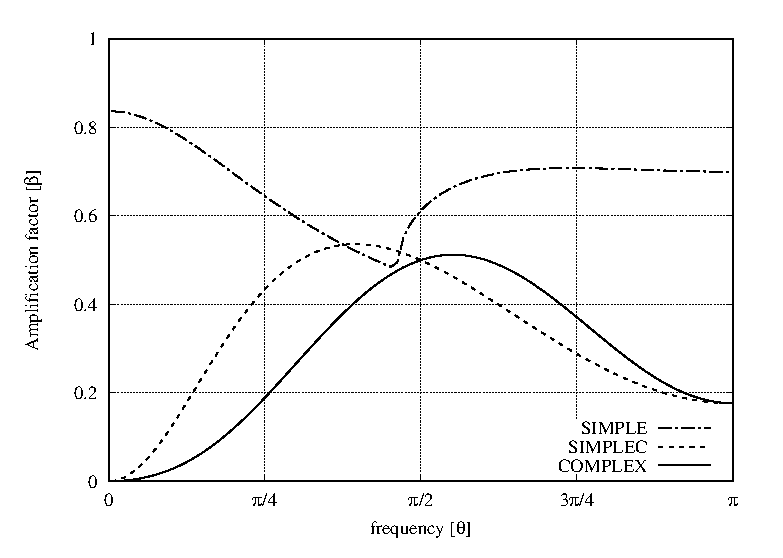
\includegraphics[width=0.49\textwidth]{fig/Re0001}
        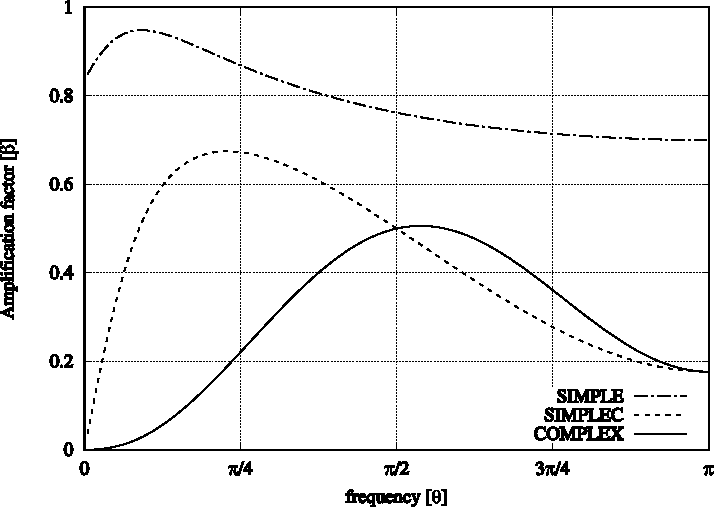
\includegraphics[width=0.49\textwidth]{fig/Re1000}
        \caption{Amplification factor for $Re_h=0.001$ (left) and $Re_h=1000$ (right)}
        \label{fig:1a}
    \end{figure}
    
    \item 2 gráficas $\beta$ vs $\theta$ con $Re=1$, SIMPLE-SIMPLEC-COMPLEX, $\omega=0.7$ y $\omega=0.95$
    
    \begin{figure}[H]
        \centering
        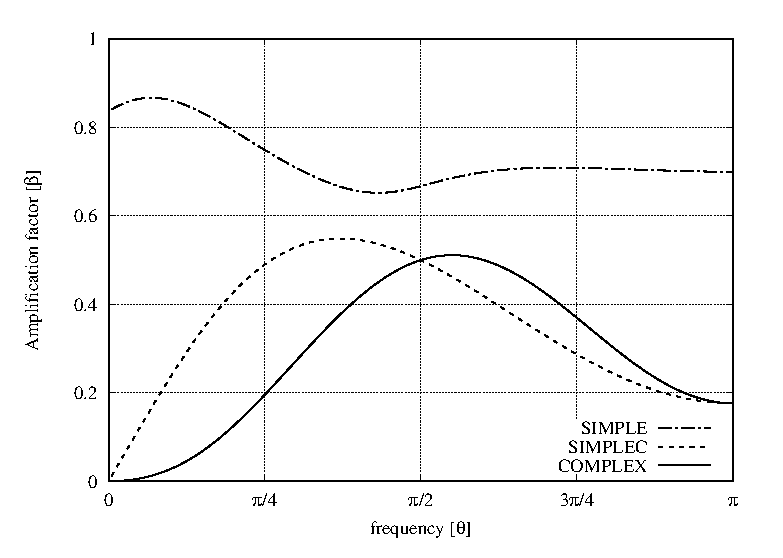
\includegraphics[width=0.49\textwidth]{fig/w07}
        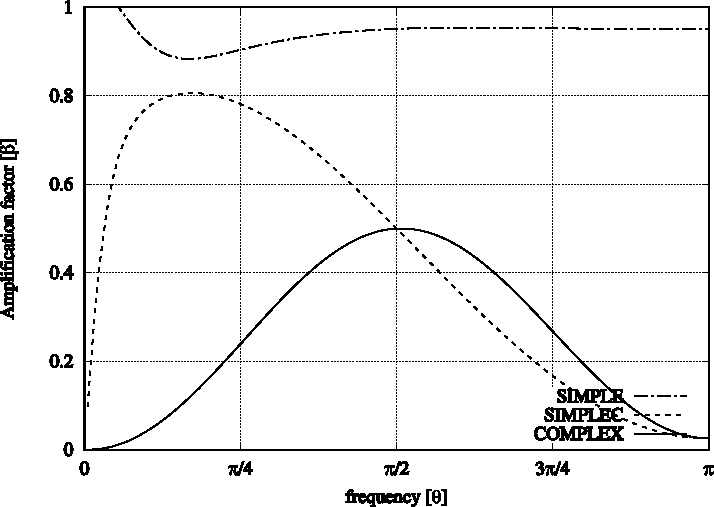
\includegraphics[width=0.49\textwidth]{fig/w095}
        \caption{Amplification factor for $\omega=0.7$ (left) and $\omega=0.95$ (right)}
        \label{fig:1b}
    \end{figure}    
    
    \item Mapas de $\beta(\theta,\omega)$, $Re=1$, SIMPLEC-COMPLEX (y SIMPLE?)
 
    \begin{figure}[H]
        \centering
        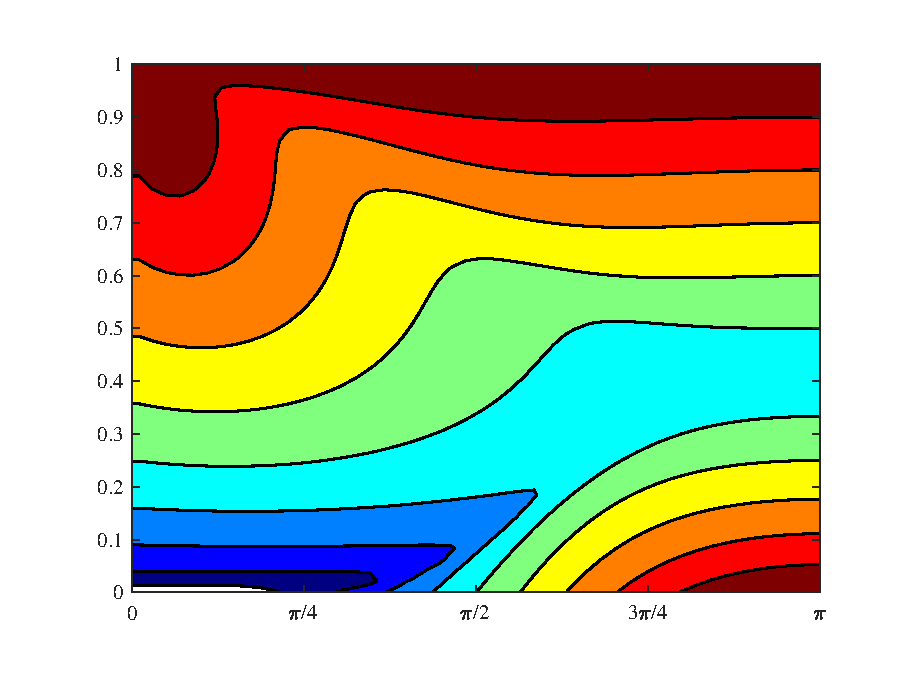
\includegraphics[width=0.6\textwidth]{fig/SIMPLE_map}
        \caption{Amplification factor for SIMPLE for different relaxation factors and frequencies}
        \label{fig:1c1}
    \end{figure}  
    \begin{figure}[H]
        \centering    
        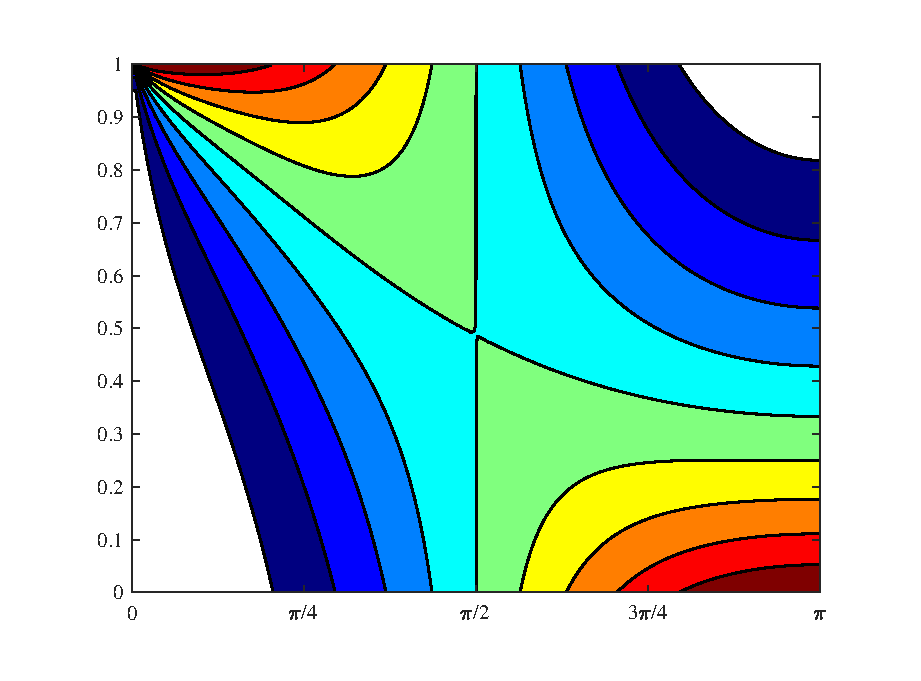
\includegraphics[width=0.6\textwidth]{fig/SIMPLEC_map}
        \caption{Amplification factor for SIMPLEC for different relaxation factors and frequencies}
        \label{fig:1c1}
    \end{figure}  
    \begin{figure}[H]
        \centering           
        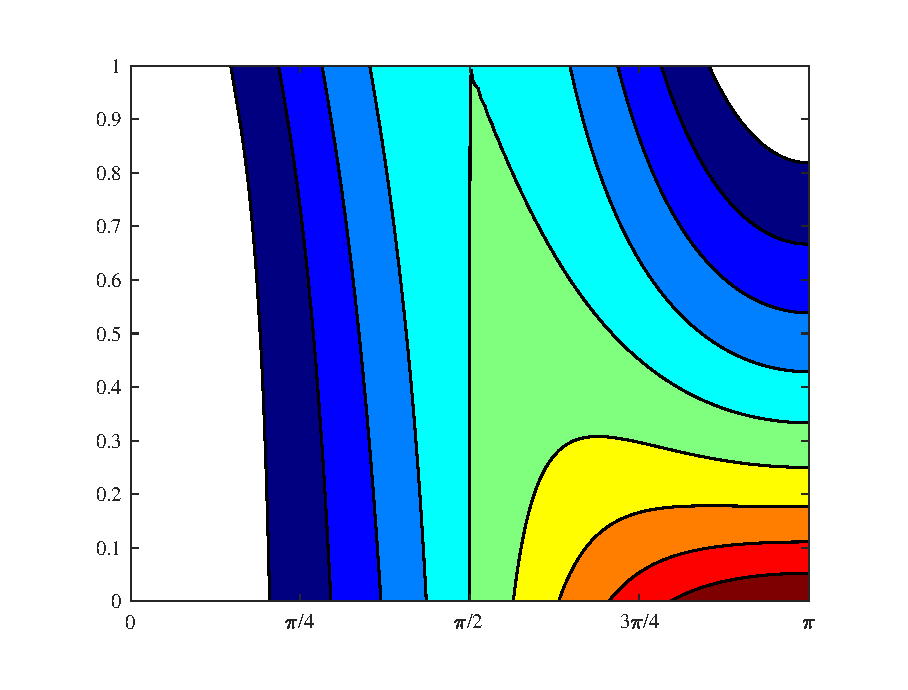
\includegraphics[width=0.6\textwidth]{fig/COMPLEX_map}
        \caption{Amplification factor for COMPLEX for different relaxation factors and frequencies}
        \label{fig:1c1}
    \end{figure}    
    
%    \begin{figure}[H]
%        \centering
%        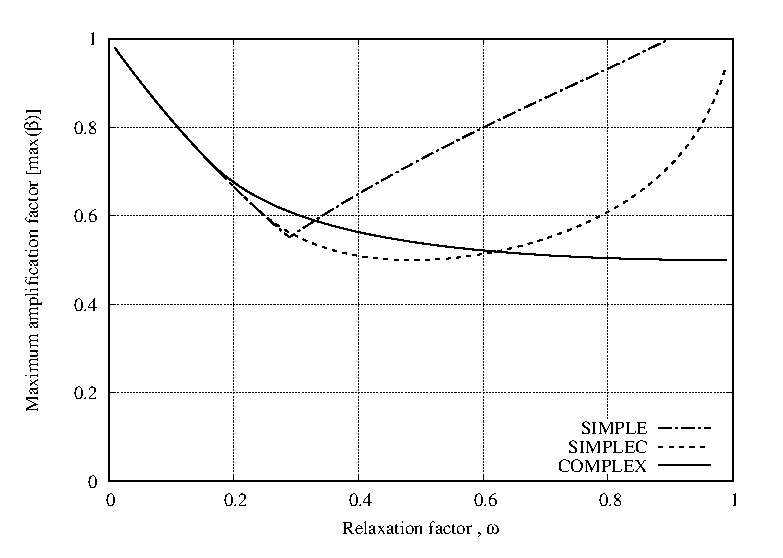
\includegraphics[width=0.7\textwidth]{fig/maxAmp}
%        \caption{Maximum amplification factor for each relaxation of momentum $\omega$}
%        \label{fig:1c}
%    \end{figure}      
    
    \item 1 gráfica $\text{mean} (\beta)$ vs $\omega$, $Re=1$, SIMPLEC-COMPLEX (y SIMPLE?)

    \begin{figure}[H]
        \centering
        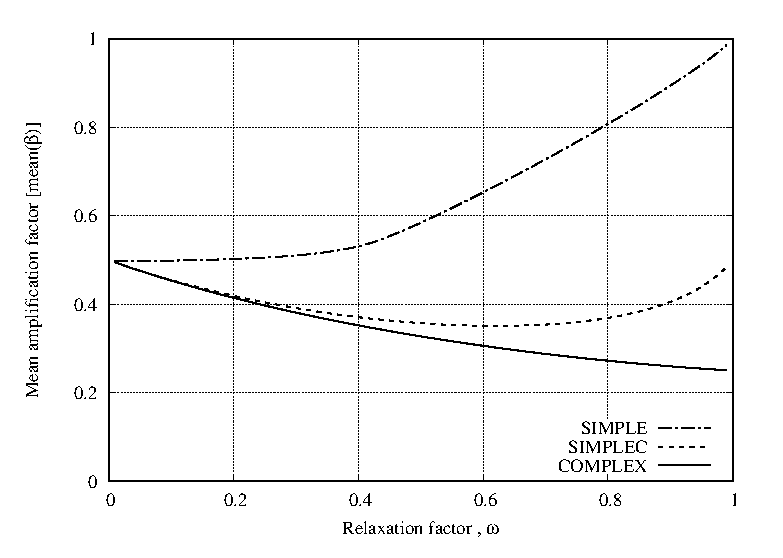
\includegraphics[width=0.6\textwidth]{fig/meanAmp}
        \caption{Mean amplification factor for each relaxation of momentum $\omega$}
        \label{fig:1d}
    \end{figure}  
    
\end{itemize}

\section{Test cases}
\label{sec:cases}

{\color{red} \subsection{Contexto general}

Flujo incompresible, laminar, estacionario.

\subsection{Metodología}

Criterio de convergencia, error,etc.

\subsection{Descripción de casos}

BFS+Cavity

\subsection{Resultados}

\begin{itemize}
    \item 4 mapas 2D (n iter vs ($\% \alpha$, $\omega_u$)) $\rightarrow$ Re altos y bajos, Cav y BFS. Conclusiones: porcentaje ideal de $\alpha$ = 0.25
    \item 12 gráficas con sombreado de n iter vs $\omega_u$ (cada una con 3 curvas: SIMPLE, SIMPLEC y COMPLEX0.25) $\rightarrow$ Re altos y bajos, malla gruesa, media y fina, Cav y BFS.
\end{itemize}

}


\section{Conclusions}
\label{sec:conclusions}

\begin{itemize}
\item A new pressure-velocity decoupling method was developed
\item The method is based on an approximation of the neighbour velocity values using a Taylor expansion
\item A stability analysis over a 1D formulation showed that the COMPLEX method is more efficient than SIMPLEC, especially for high relaxation factors.
\tiem 
\end{itemize}

\bibliographystyle{plain}
\bibliography{main}

\end{document}
